\documentclass[tikz,border=10pt]{standalone}
\usepackage{pgfplots}
\pgfplotsset{compat=1.18}

\begin{document}
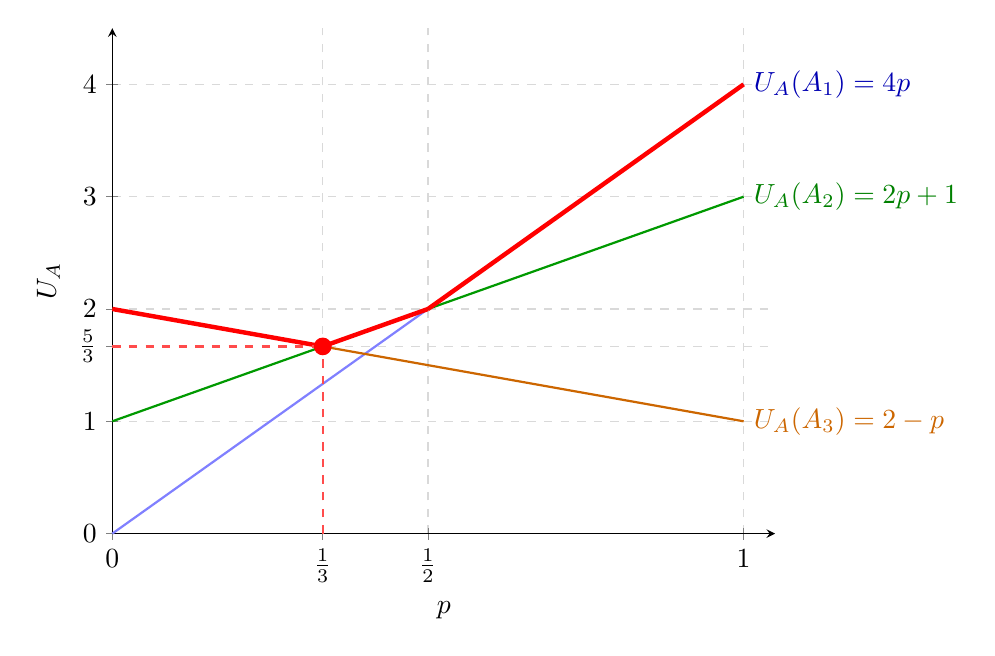
\begin{tikzpicture}
\begin{axis}[
    axis lines = left,
    xlabel = {$p$},
    ylabel = {$U_A$},
    xmin = 0, xmax = 1.05,
    ymin = 0, ymax = 4.5,
    xtick = {0, 0.333, 0.5, 1},
    xticklabels = {$0$, $\frac{1}{3}$, $\frac{1}{2}$, $1$},
    ytick = {0, 1, 1.667, 2, 3, 4},
    yticklabels = {$0$, $1$, $\frac{5}{3}$, $2$, $3$, $4$},
    grid = both,
    grid style = {dashed, gray!30},
    clip = false,
    width = 10cm,
    height = 8cm
]

    % Base lines with labels placed at the right endpoint (p = 1)
    \addplot[domain=0:1, samples=2, blue!50, thick] {4*x}
        node[pos=1, right, blue!70!black] {$U_A(A_1) = 4p$};

    \addplot[domain=0:1, samples=2, green!60!black, thick] {2*x + 1}
        node[pos=1, right, green!50!black] {$U_A(A_2) = 2p + 1$};

    \addplot[domain=0:1, samples=2, orange!80!black, thick] {2 - x}
        node[pos=1, right, orange!80!black] {$U_A(A_3) = 2 - p$};

    % Highlight Upper Envelope (Max for each p) in Red
    \addplot[domain=0:1/3, samples=2, red, ultra thick] {2 - x};
    \addplot[domain=1/3:1/2, samples=2, red, ultra thick] {2*x + 1};
    \addplot[domain=1/2:1, samples=2, red, ultra thick] {4*x};

    % Minimax point only
    \addplot[only marks, mark=*, mark size=3pt, red] coordinates {(1/3, 5/3)};
    \node[above, red, font=\small] at (axis cs:1/3, 1.75) {};

    % Dashed guidelines for minimax point
    \draw[dashed, red!70, thick] (axis cs:1/3, 0) -- (axis cs:1/3, 5/3);
    \draw[dashed, red!70, thick] (axis cs:0, 5/3) -- (axis cs:1/3, 5/3);

\end{axis}
\end{tikzpicture}
\end{document}
